\graphicspath{{figures/chap04/}}

\chapter{SUNIST 氦放电等离子体的发射光谱诊断}
\label{chap:experiment}

本章首先给出 SUNIST 氦放电等离子体原子发射谱线强度的测量结果,利用谱线比法诊断了氦等离子体的 $T_{\rm e}$ 和 $N_{\rm e}$,将诊断结果与微波干涉仪测量的弦平均电子密度进行对比以验证谱线比法的适用性,%在实验条件下,
通过对比激发态数密度实际测量与模型的计算结果对碰撞辐射模型进行了再次核验。最后,分析了由光谱测量弦积分特性带来的问题,并初步研究了谱线强度涨落蕴含的等离子体行为信息,为今后丰富和发展 SUNIST 光谱诊断工作提供了一些参考。%磁流体并给出一种可以用于定性诊断 SUNIST 电子密度参数分布的方法。

\section{氦原子发射谱线强度测量结果}
\label{sec:chap04:sunist-spec-measurements}

\begin{figure}%[H]
	\centering
%    \begin{subfigure}{0.51\columnwidth}
        \begin{overpic}[width=0.5\columnwidth]{he-ip-and-vlight-for-gpxygpfx.pdf}
            \put(30,0){\mbox{\colorbox{white}{\hspace{1.5em}时间 (ms)\hspace{2.5em}}}}
            \put(-2,30){\rotatebox{90}{\mbox{\colorbox{white}{$I_{\rm p}$ ($\rm kA$)\quad}}}}
            \put(93,30){\rotatebox{90}{\mbox{\colorbox{white}{V.L. (a.u.)\quad}}}}
        \end{overpic}
%        %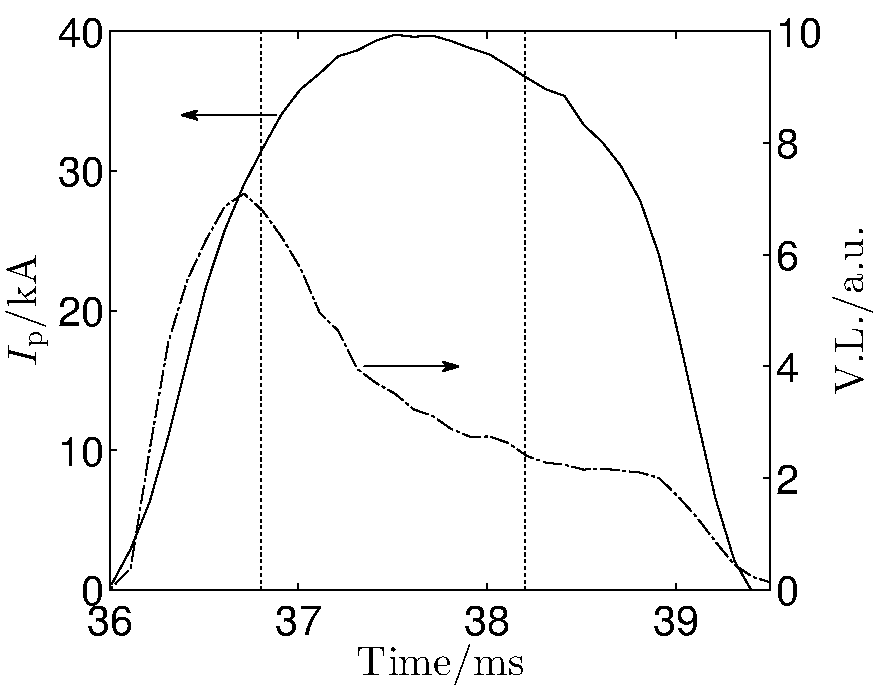
\includegraphics[width=\columnwidth]{he-ip-and-vlight-for-gpxygpfx.pdf}
%        \caption{等离子体电流($I_{\rm p}$)与可见光辐射(V.L.)}%
%        \label{fig:chap04:ip-vlight}
%    \end{subfigure}
%%    \hspace{0.04\textwidth}
%    \begin{subfigure}{0.43\columnwidth}
%        \begin{overpic}[width=\columnwidth]{he-line-gasss-fit-447-at-37ms.pdf}
%            \put(33,0){\mbox{\colorbox{white}{\hspace{1.5em}$\Delta\lambda$ (\AA)\hspace{2.5em}}}}
%            \put(-2,35){\rotatebox{90}{\mbox{\colorbox{white}{$I$ (a.u.)\quad}}}}
%            %\put(93,30){\rotatebox{90}{\mbox{\colorbox{white}{V.L. (a.u.)\quad}}}}
%        \end{overpic}
%        %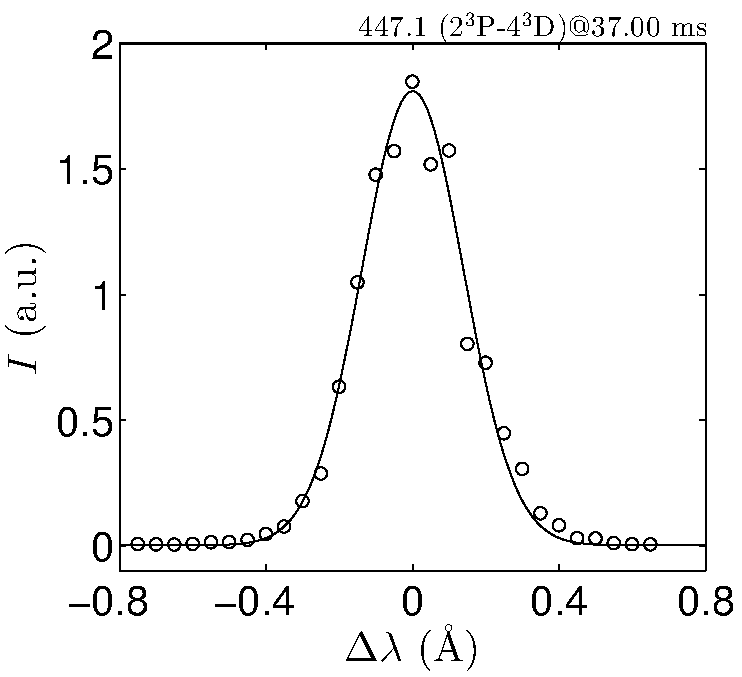
\includegraphics[width=\columnwidth]{he-line-gasss-fit-447-at-37ms.pdf}
%        \caption{谱线高斯拟合,以 $447.1\,{\rm nm}$ 线为例}%
%        \label{fig:chap04:line-shape}
%    \end{subfigure}
	\caption{SUNIST 氦放电等离子体电流($I_{\rm p}$)与可见光辐射(V.L.)信号。图片来自 \onlinecite{xie:wlxb}。}
	\label{fig:chap04:ip-vlight}
\end{figure}

图 \ref{fig:chap04:ip-vlight} 显示的是氦气欧姆放电时等离子体电流与可见光辐射波形。SUNIST 中心柱空间狭窄,欧姆场加热能力受到极大限制,欧姆放电等离子体电流平顶段时间很短\cite{TanYi2008:Thesis},但是,我们仍然可以将准稳态的碰撞辐射模型计算结果应用于平顶段等离子体的 $T_{\rm e}$ 和 $N_{\rm e}$ 诊断。因为碰撞辐射模型是对等离子体原子反应过程的描述,衡量等离子体内原子碰撞辐射过程是否可以在局部区域内达到准稳态的标准即为第 \ref{sec:chap03:quasi-stationary} 节提到的各过程时间常数的对比。

王文浩等人\cite{WangWH2005:PPCF:Edge}对 SUNIST 欧姆放电边界输运行为的研究发现,等离子体涨落由中心区域向边界输运,其径向输运相速度 $v_{{\rm ph}r}$ 在刮削层为 $v_{{\rm ph}r}\sim0.7\,{\rm km}/{\rm s}$、在等离子体边界区域为 $v_{{\rm ph}r}\sim0.9-1.4\,{\rm km}/{\rm s}$,而 SUNIST 等离子体小半径 $a\sim0.23\,{\rm m}$,由此我们估算 SUNIST 等离子体在空间上的输运时间常数 $\tau_{\rm plasma}\sim0.3\,{\rm ms}$。将式 (\ref{eq:chap03:time-constant-compare}) 更加具体地写出:
\begin{equation}
\label{eq:chap04:time-constant-compare}
    \tau_{\rm ord-rad}\sim0.01\,\mu{\rm s}\ll
    \tau_{\rm e-e,i-i}\sim4-20\,\mu{\rm s}\ll
    \tau_{\rm ion}\sim1.4-140\,\mu{\rm s}\ll
    \tau_{\rm plasma}\sim300\,\mu{\rm s}
\end{equation}
可见,对于 SUNIST 放电平顶段等离子体,在局部区域内的等离子体原子反应过程中,可以忽略由等离子体输运等行为带来的等离子体参数变化,将准稳态的碰撞辐射模型计算结果应用在光谱诊断中。

由图 \ref{fig:chap04:ip-vlight} 所示,根据等离子体能量平衡和放电时的碰撞辐射反应过程,我们还可以做出以下定性分析:在放电起始阶段,工作气体被电离并约束在磁场中形成等离子体电流,此时大量原子被激发并产生辐射,可见光信号快速上升,等离子体处于电离过程大于复合过程的状态,碰撞辐射过程未达到平衡;当可见光开始下降时,虽然等离子体电流尚未进入平顶阶段,但等离子体内的碰撞辐射过程开始趋于平衡;等离子体平顶段过后,欧姆场加热能力减弱,等离子体电流开始下降,此时的复合过程开始逐渐增大,碰撞辐射平衡也被破坏。

本文稳态情况下的碰撞模型只适合如图 \ref{fig:chap04:ip-vlight} 所示虚线中间放电段的等离子体,这也是 SUNIST 等离子体可以用来进行托卡马克物理研究的放电时段。
在放电起始和结束阶段,除了需要对碰撞辐射模型速率方程进行含时求解外,其他一些因素的影响也是不可忽略的,在第 \ref{sec:chap06:buzuhezhanwang} 节中将给出相应讨论。

\begin{table}%[H]
\caption{本文测量氦原子谱线的跃迁、波长和有效自发辐射跃迁速率系数\cite{xie:wlxb}}
\label{table:chap04:helines}
\begin{center}
\begin{tabular}{cC{7em}c}\toprule[1.5pt]
跃迁 & \makecell[c]{$\lambda_{q\to p}$ (${\rm nm})$} & \makecell[c]{$A_{q\to p}^{\rm eff}$ ($10^7\,{\rm s}^{-1}$)}\\
\midrule[1pt]
$2^1{\rm S}\leftarrow3^1{\rm P}$ & 501.6 & 1.34 \\
$2^1{\rm S}\leftarrow4^1{\rm P}$ & 396.5 & 0.70 \\
$2^1{\rm P}\leftarrow4^1{\rm S}$ & 504.8 & 0.68 \\
$2^1{\rm P}\leftarrow4^1{\rm D}$ & 492.2 & 1.99 \\
$2^3{\rm S}\leftarrow3^3{\rm P}$ & 388.9 & 0.95 \\
$2^3{\rm P}\leftarrow3^3{\rm D}$ & 587.6 & 7.07 \\
$2^3{\rm P}\leftarrow4^3{\rm S}$ & 471.3 & 0.95 \\
$2^3{\rm P}\leftarrow4^3{\rm D}$ & 447.1 & 2.46 \\
$2^3{\rm P}\leftarrow5^3{\rm S}$ & 412.1 & 0.45 \\
\bottomrule[1.5pt]
\end{tabular}
\end{center}
\end{table}


氦原子从 $q$ 能级跃迁至 $p$ 能级时,发出波长为 $\lambda_{qp}$ 的谱线,该谱线的光子数辐射率 $\epsilon_{qp}$ 为:
\begin{eqnarray}
\epsilon_{qp}=\left(4\pi\right)^{-1}N_qA_{qp}
\end{eqnarray}
其中,$N_q$ 为跃迁高能级 $q$ 的粒子数密度,$A_{qp}$ 为爱因斯坦系数,即自发跃迁速率系数。单色仪测得的光信号强度为沿观察路径 $L$ 的等离子体线辐射积分:
\begin{eqnarray}
I_{\lambda_{qp}}=R_{\rm M}\int_LT_{\lambda_{qp}}\epsilon_{qp}\Omega_lS\,{\rm d}l
\end{eqnarray}
其中,$R_{\rm M}$ 为单色仪 ${\rm M}$ 的响应,$T_{\lambda_{qp}}$ 为线辐射在等离子体中的传播系数,$S\,{\rm d}l$ 与 $\Omega_l$ 分别为在观察路径 $l$ 处等离子体的体积与光纤入口平面所呈的立体角。光纤与等离子体的相对位置固定,并考虑氦原子谱线的精细结构,所以:
\begin{eqnarray}
\label{eq:lineintensity}
I_{\lambda_{qp}}=R_{\rm M}T_{\lambda_{qp}}A_{qp}^{\rm eff}\overline{N_q}L
\end{eqnarray}
其中,$\overline{N_q}$ 为 $q$ 激发态的弦平均密度,$A_{qp}^{\rm eff}$ 为有效自发辐射跃迁速率系数:
\begin{eqnarray}
A_{qp}^{\rm eff}=\frac{1}{g_q}\sum_mg_mA_{qp}^m
\end{eqnarray}
其中,$m$ 表示第 $m$ 条精细谱线,$g_q$ 与 $g_m$ 为 $q$ 能级的总统计权重与辐射第 $m$ 条精细谱线的 $q$ 能级的统计权重,而爱因斯坦系数 $A_{qp}^{m}$ 可以通过查表得到\cite{NISTdatabase}。本文测量使用了氦原子在可见光波段的原子谱线,其能级跃迁,波长与有效自发辐射速率系数如表 \ref{table:chap04:helines} 所示。

\begin{figure}%[H]
  \centering
  \begin{overpic}[width=0.8\textwidth]{he-lines-whole-intensity-calibrated.pdf}
    \put(40,1){\mbox{\colorbox{white}{\hspace{1.5em}时间 ($\rm ms$)\hspace{2.5em}}}}
    \put(0,40){\rotatebox{90}{\mbox{\colorbox{white}{$I$ (a.u.)\quad}}}}
    %\put(93,30){\rotatebox{90}{\mbox{\colorbox{white}{V.L. (a.u.)\quad}}}}
  \end{overpic}
  %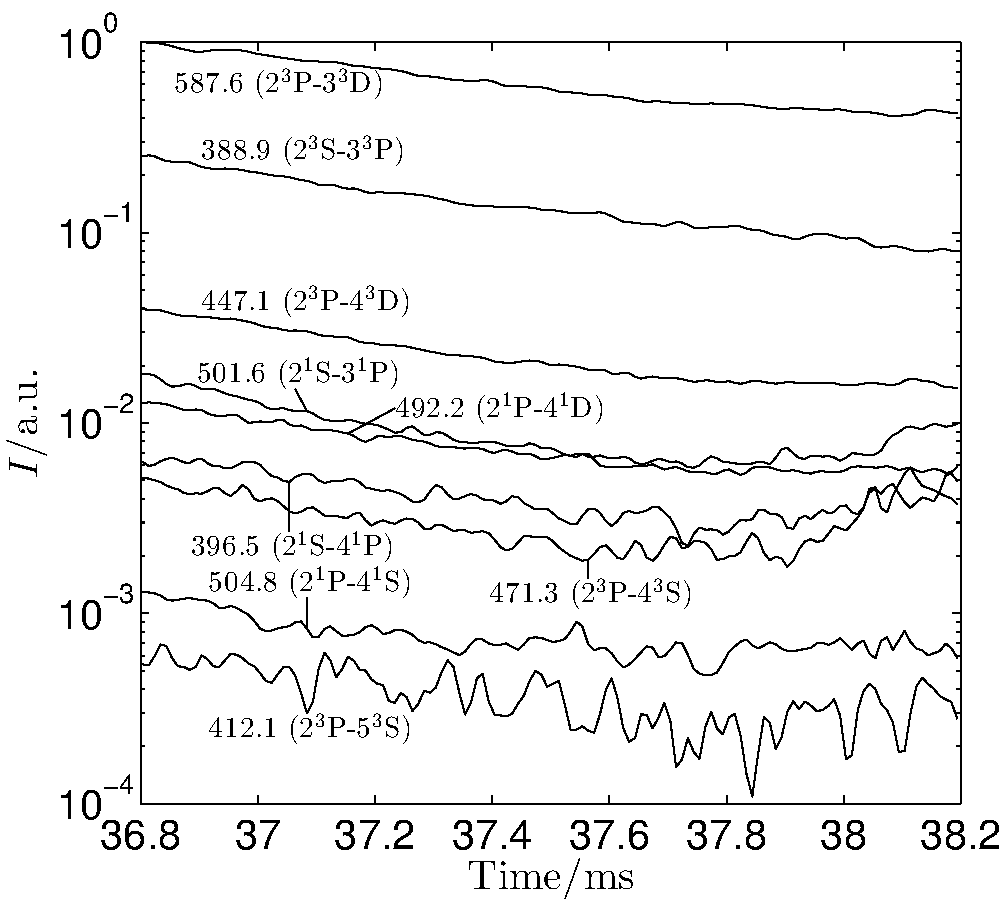
\includegraphics[width=0.8\textwidth]{he-lines-whole-intensity-calibrated.pdf}
  \caption{SUNIST 氦放电等离子体的原子谱线强度测量结果。图片来自 \onlinecite{xie:wlxb}。}
  \label{fig:chap04:he-lines-all}
\end{figure}

表 \ref{table:chap04:helines} 中谱线的相对强度在平顶段随时间的变化在图 \ref{fig:chap04:he-lines-all} 中画出。氦原子谱线强度随时间的变化与可见光有相同的趋势,其强度之间最大有三个数量级的差别。

\section{谱线比法诊断 $T_{\rm e}$ 和 $N_{\rm e}$}
\label{sec:chap04:lineratio-ne-te}

%\subsection{与微波干涉仪和静电探针诊断结果的对比}

\begin{figure}%[H]
  \centering
  \begin{overpic}[width=0.7\textwidth]{lineratio-te-ne-soliderrorbar.pdf}
    \put(30,1){\mbox{\colorbox{white}{\hspace{1.5em}时间 ($\rm ms$)\hspace{2.5em}}}}
    \put(0,23){\rotatebox{90}{\mbox{\colorbox{white}{$T_{\rm e}$ ($\rm eV$)\quad}}}}
    \put(79,17){\rotatebox{90}{\mbox{\colorbox{white}{\color{red}$N_{\rm e}$ $(\times10^{12}\,{\rm cm}^{-3})$\quad}}}}
  \end{overpic}
  %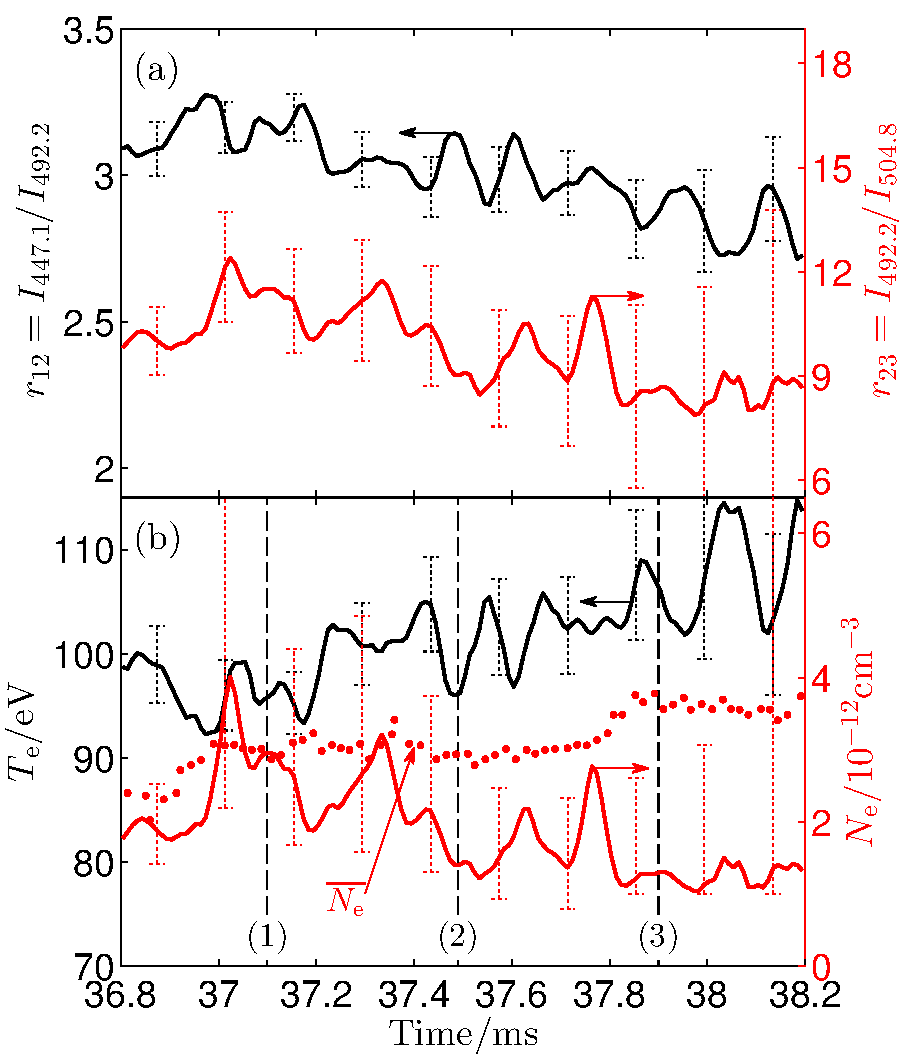
\includegraphics[width=0.6\textwidth]{lineratio-te-ne.pdf}
  \caption{谱线比法确定 SUNIST 等离子体参数。(a):两谱线强度比;(b):谱线强度比确定的 $T_{\rm e}$ 与 $N_{\rm e}$ 参数,以
及 $94\,{\rm GHz}$ 微波干涉仪测量的赤道面上弦平均电子密度 $\overline{N_{\rm _e}}$。图片来自 \onlinecite{xie:wlxb}。}
  \label{fig:chap04:lineratio-te-ne}
\end{figure}

电子温度 $T_{\rm e}$ 敏感谱线强度比 $r_{12}=I_{447.1}/I_{492.2}$ 与电子密度 $N_{\rm e}$ 敏感谱线比 $r_{23}=I_{492.2}/I_{504.8}$ 的计算结果如图 \ref{fig:chap04:lineratio-te-ne}(a) 所示。根据第 \ref{sec:chap03:lineratio-method} 节碰撞辐射模型计算的谱线比等高线与同时确定 $T_{\rm e}$ 和 $N_{\rm e}$ 的谱线比法得到的参数在图 \ref{fig:chap04:lineratio-te-ne}(b) 中画出;%其中,$T_{\rm e}$ 和 $N_{\rm e}$ 诊断误差由第 \ref{sec:chap03:lineratio-error-to-result-error} 节固定另外一个谱线比的条件误差计算给出;
另外, $94\,{\rm GHz}$ 微波干涉仪测量的弦平均电子密度 $\overline{N_{\rm e}}$ 结果也在图 \ref{fig:chap04:lineratio-te-ne}(b) 中画出。可以看出,氦原子谱线比法与微波干涉仪对电子密度的诊断结果相吻合,由此,本文所建立的氦原子谱线比法诊断初步得到了验证。

我们注意到,谱线比法对 $N_{\rm e}$ 的诊断略低于微波干涉仪的诊断结果,其原因将在第 \ref{sec:chap04:chord-integration} 节进行详细分析。在测量结果中,谱线强度的涨落造成了谱线比的涨落,从而导致等离子体参数诊断结果的涨落,而谱线强度的涨落包含了等离子体磁流体力学的信息,在第 \ref{sec:chap04:line-dbp10-fluctuation} 节中,我们将对此进行初步分析。

\section{氦原子碰撞辐射模型的复核}
\label{sec:chap04:rel-levelabun-crm-to-exp}

在谱线比法获得的等离子体 $T_{\rm e}$ 和 $N_{\rm e}$ 参数下,利用碰撞辐射模型计算出表 \ref{table:chap04:helines} 中实验测量的谱线激发态能级的数密度 $N_q^{\rm crm}/g_q$,其中 $g_q$ 为谱线上能级 $q$ 的统计权重。

根据式 (\ref{eq:lineintensity}),实验测量的激发态弦平均相对密度为:
\begin{eqnarray}
N_q^{\rm exp}/g_q=CI_{\lambda_{qp}}\left(T_{\lambda_{qp}}R_{\rm M}A_{qp}^{\rm eff}\right)^{-1}/g_q
\end{eqnarray}
其中,$C$~为归一化因子。

图 \ref{fig:chap04:RelLevelabunAt3Times} 分别显示了在 $37.10\,{\rm ms}$、$37.49\,{\rm ms}$ 与 $37.90\,{\rm ms}$ 三个时刻实验测量与碰撞辐射模型计算的各能级相对数密度,在 SUNIST 整个放电平顶段中,实验测量与碰撞辐射模型计算的氦原子能级数密度之间的对比由图 \ref{fig:chap04:RelLevelabunCRMtoEXP} 给出。从实验和碰撞辐射模型给出结果的对比可以得出,碰撞辐射模型能很好的对等离子体中各能级的相对数密度进行预测,从而通过实验数据对碰撞辐射模型再次进行了核对,验证了本文建立的碰撞辐射模型对 SUNIST 氦放电等离子体的适用性。

\begin{figure}%[H]
    \centering
    \begin{overpic}[width=\textwidth]{rel_levelabun-at-three-times.pdf}
    %\put(22.5,1.5){\mbox{\colorbox{white}{\hspace{1.5em}时间}}}
    %\put(0,23){\rotatebox{90}{\mbox{\colorbox{white}{$T_{\rm e}$ ($\rm eV$)\quad}}}}
    \put(-0.2,19){\rotatebox{90}{\mbox{\colorbox{white}{\hspace{0.2em}(a.u.)}}}}
    \put(96,19){\rotatebox{90}{\mbox{\colorbox{white}{\hspace{0.2em}(a.u.)}}}}
    \end{overpic}
    %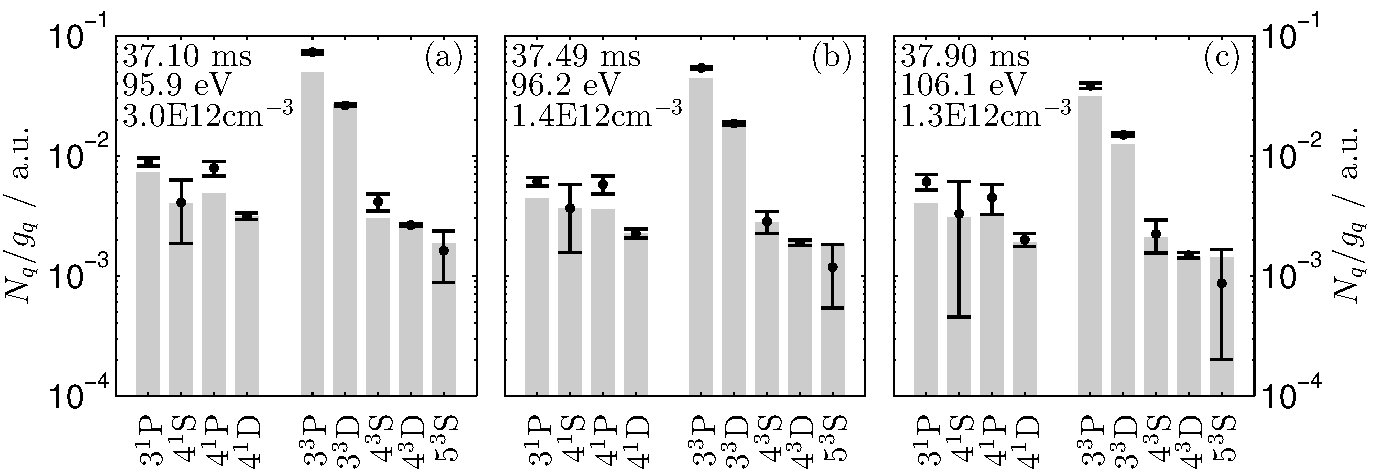
\includegraphics[width=\textwidth]{rel_levelabun-at-three-times.pdf}
    \caption{氦原子谱线对应激发态的相对数密度。(a)、(b) 和 (c) 分别对应图\ref{fig:chap04:lineratio-te-ne} 中 (1)、(2) 和 (3) 时刻的激发态相对数密度。\textbullet:实验测量值;{\color{gray}\RectangleBold}:碰撞辐射模型计算值。图片来自 \onlinecite{xie:wlxb}。}%
    \label{fig:chap04:RelLevelabunAt3Times}
\end{figure}

\begin{figure}%[H]
    \centering
    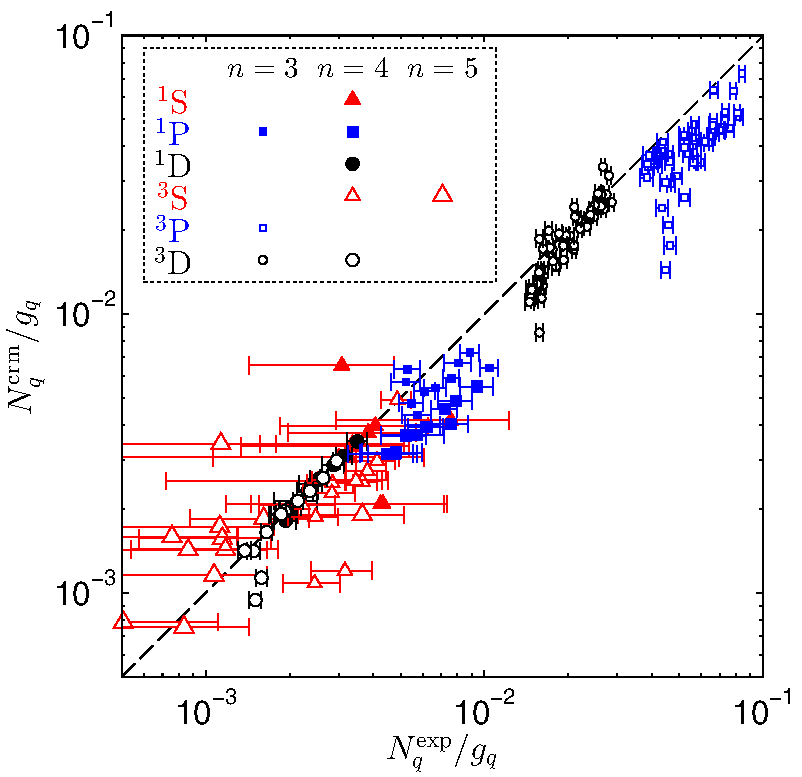
\includegraphics[width=0.8\textwidth]{rel_levelabun-crm-to-exp.pdf}
    \caption{氦原子激发态相对数密度碰撞辐射模型计算值~$N_q^{\rm crm}/g_q$~与实验测量值~$N_q^{\rm exp}/g_q$~ 的比较。图片来自 \onlinecite{xie:wlxb}。}%
    \label{fig:chap04:RelLevelabunCRMtoEXP}
\end{figure}

因为自旋单重态的数密度主要对 $N_{\rm e}$ 敏感,而自旋三重态数密度主要对 $T_{\rm e}$ 敏感,图 \ref{fig:chap04:RelLevelabunAt3Times} 中能级以自旋单重态和自旋三重态被分为两组。图 \ref{fig:chap04:RelLevelabunAt3Times}(a) 与图 \ref{fig:chap04:RelLevelabunAt3Times}(b) 的对比说明在 $N_{\rm e}$ 较高时自旋单重态的数密度增加,而碰撞辐射模型计算的 $3^1{\rm P}$ 与$4^1{\rm P}$ 能级粒子数密度增加幅度大于 $4^1{\rm S}$ 和 $4^1{\rm D}$ 能级。在 SUNIST 等离子体参数下,氦原子自旋单重态能级的主要直接来源为基态原子的碰撞激发,从图 \ref{fig:chap04:excRateForLines}(a) 中可以看出,$3^1{\rm P}$ 与 $4^1{\rm P}$ 能级的基态碰撞激发速率系数远大于 $4^1{\rm S}$ 和 $4^1{\rm D}$ 能级,所以电子密度 $N_{\rm e}$ 对 $3^1{\rm P}$ 与 $4^1{\rm P}$ 能级数密度的影响更加明显。图 \ref{fig:chap04:RelLevelabunAt3Times}(b) 与图 \ref{fig:chap04:RelLevelabunAt3Times}(c) 的对比说明在 $T_{\rm e}$ 较高时碰撞辐射模型对除 $3^3{\rm P}$ 之外的自旋三重态的数密度计算结果相对实验测量有所降低。此时,图 \ref{fig:chap04:RelLevelabunAt3Times} 所示自旋三重态能级的主要直接来源为亚稳态 $2^3{\rm S}$ 能级的碰撞激发,而除 $3^3{\rm P}$ 外的自旋三重态能级的碰撞激发速率系数随 $T_{\rm e}$ 的上升而下降(图 \ref{fig:chap04:excRateForLines}(b))。

\begin{figure}%[H]
    \centering
    \begin{overpic}[width=0.6\textwidth]{excRate-for-rel-levelabun.pdf}
    \put(40,1){\mbox{\colorbox{white}{\small $T_{\rm e}$ ($\rm eV$)}}}
    \put(0.5,20){\rotatebox{90}{\mbox{\colorbox{white}{\small $C_{2q}$ (${\rm cm}^{-3}$)\quad}}}}
    \put(0,65){\rotatebox{90}{\mbox{\colorbox{white}{\small $C_{1q}$ (${\rm cm}^{-3}$)\quad}}}}
    \end{overpic}
    %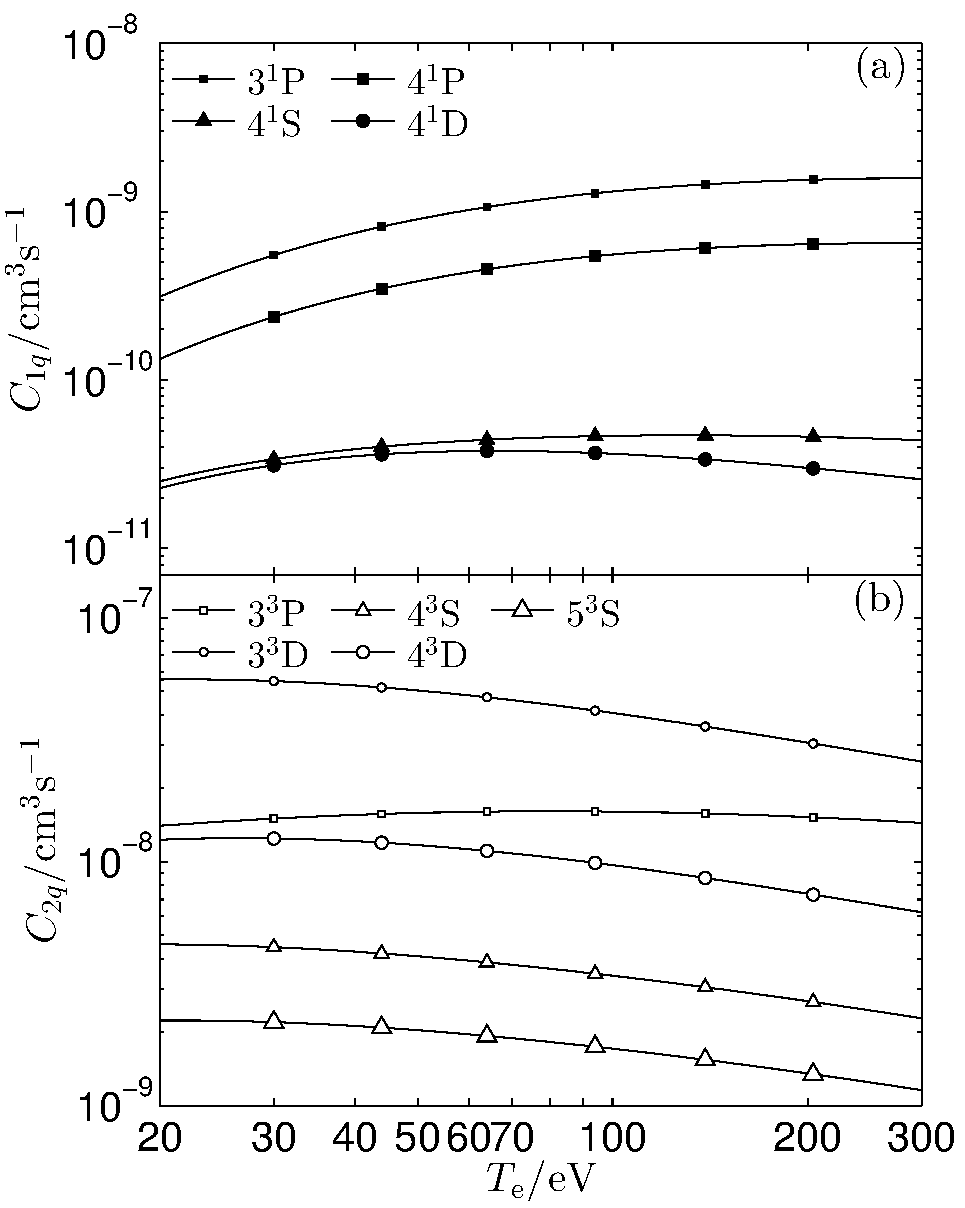
\includegraphics[width=0.6\textwidth]{excRate-for-rel-levelabun.pdf}
    \caption{氦原子的激发速率系数。 (a) 基态 $1^1{\rm S}$ 激发;(b) 亚稳态 $2^3{\rm S}$ 激发。图片来自 \onlinecite{xie:wlxb}。}%
    \label{fig:chap04:excRateForLines}
\end{figure}

图 \ref{fig:chap04:RelLevelabunAt3Times} 与图 \ref{fig:chap04:RelLevelabunCRMtoEXP} 还显示,$3^1{\rm P}$、$4^1{\rm P}$ 与 $3^3{\rm P}$ 能级的碰撞辐射模型计算结果低于实验测量值。这三个能级所对应的谱线辐射跃迁低能级为 $2^1{\rm S}$ 或 $2^3{\rm S}$ 亚稳态(表 \ref{table:chap04:helines}),由于亚稳态的粒子数比其他激发态要高很多,$3^1{\rm P}$、$4^1{\rm P}$ 与 $3^3{\rm P}$ 三个能级的谱线辐射具有较高的再吸收系数\cite{boivin2001,Boivin2007},导致这三个能级数密度的增长,而我们建立的碰撞辐射模型中忽略了再吸收的影响,在实际工作中,人们一般不选择这些谱线进行诊断研究。

\section{光谱测量的弦积分特性与谱线强度涨落的初步研究}

\subsection{光谱测量弦积分特性的研究}
\label{sec:chap04:chord-integration}

实验测量的谱线辐射积分强度结果反应的是沿观察弦的平均激发态能级数密度。使用碰撞模型对激发态能级估计时,先采用三条谱线的弦积分强度比确定出等离子体参数后,再计算激发态的能级数密度。计算过程中包含了一个假设,即弦平均光谱强度比得出的 $T_{\rm e}$ 和 $N_{\rm e}$ 参数等于弦平均的电子参数。而氦原子的谱线辐射强度与电子温度和密度之间并非线性关系,利用弦平均氦原子谱线辐射强度比诊断的电子密度与微波干涉仪测量的弦平均电子密度会有差别(图 \ref{fig:chap04:lineratio-te-ne})。

\begin{figure}%[H]
    \centering
    \begin{overpic}[width=.6\textwidth]{ne-te-and-line-intensity-profile.pdf}
    %\put(22.5,1.5){\mbox{\colorbox{white}{\hspace{1.5em}时间}}}
    %\put(0,23){\rotatebox{90}{\mbox{\colorbox{white}{$T_{\rm e}$ ($\rm eV$)\quad}}}}
    \put(-0.2,25){\rotatebox{90}{\mbox{\colorbox{white}{$I$ (a.u.)}}}}
    %\put(96,19){\rotatebox{90}{\mbox{\colorbox{white}{\hspace{0.2em}(a.u.)}}}}
    \end{overpic}
    %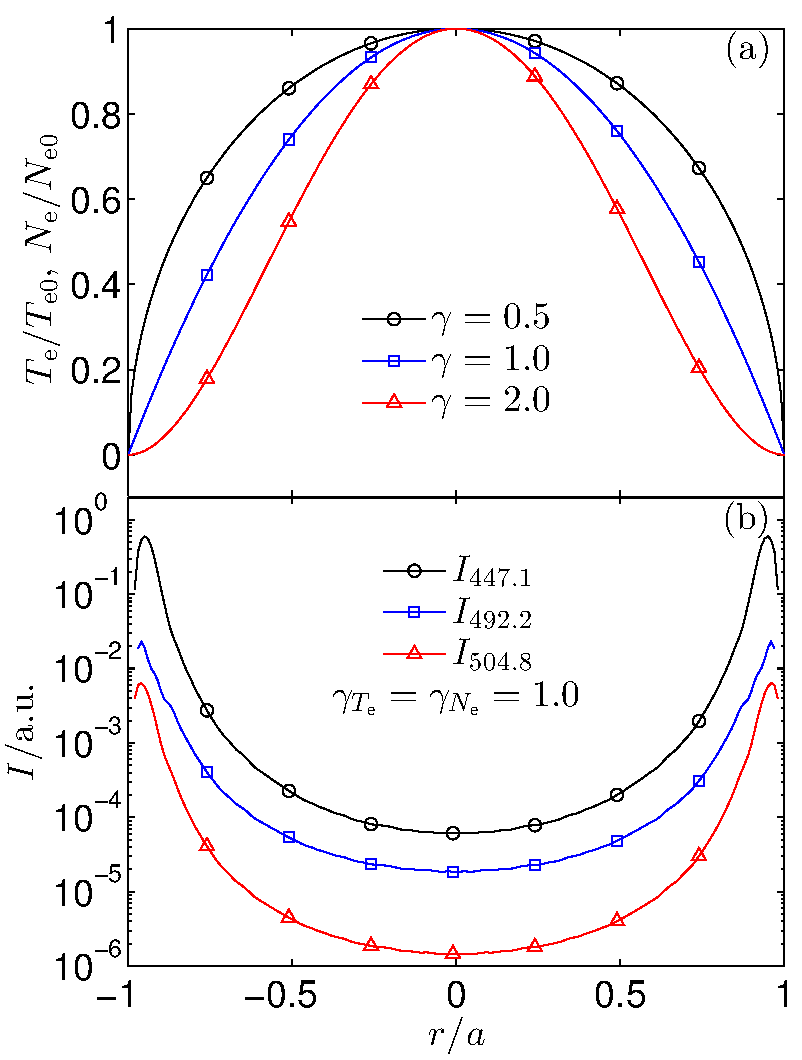
\includegraphics[width=.6\textwidth]{ne-te-and-line-intensity-profile.pdf}
    \caption{(a):不同抛物线分布参数 $\gamma$ 下的 $T_{\rm e}$ 与 $N_{\rm e}$ 分布;(b):分布参数 $\gamma_{T_{\rm e}}=\gamma_{N_{\rm e}}=1.0$ 时,三条氦原子谱线辐射强度的分布。}%
    \label{fig:chap04:ne-te-and-line-intensity-profile}
\end{figure}

要定量分析此假设对碰撞辐射模型计算结果引起的误差,需要对等离子体进行空间分辨诊断。目前,SUNIST 尚不具备 $T_{\rm e}$ 与 $N_{\rm e}$ 的空间分辨诊断能力。根据文献 \onlinecite{Fujimoto1989:NF} 的处理方法,不妨假设 $T_{\rm e}$ 与 $N_{\rm e}$ 为抛物线分布,即:
\begin{align}
N_{\rm e}=N_{\rm e,0}\left[1-(r/a)^2\right]^{\gamma_{N_{\rm e}}}\\
T_{\rm e}=T_{\rm e,0}\left[1-(r/a)^2\right]^{\gamma_{T_{\rm e}}}
\end{align}
其中,$r$ 为径向位置,$a$ 为小半径(为了简化,包含阴影区在内),$N_{\rm e,0}$ 和 $T_{\rm e,0}$ 为等离子体中心的电子密度和温度,$\gamma_{N_{\rm e}}$ 和 $\gamma_{T_{\rm e}}$ 分别为电子密度和温度分布参数。

\begin{figure}%[H]
    \centering
    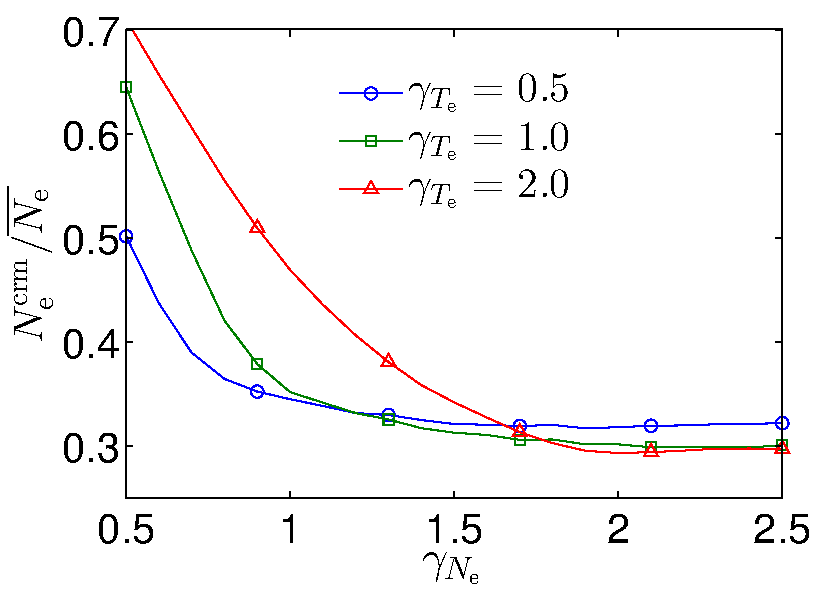
\includegraphics[width=.6\textwidth]{line-int-ratio-params-to-mean-ne.pdf}
    \caption{谱线比法获得的 $N_{\rm e}^{\rm crm}$ 与微波干涉仪获得的弦平均电子密度 $\overline{N_{\rm e}}$ 比值随电子密度分布参数 $\gamma_{N_{\rm e}}$ 的变化。}%
    \label{fig:chap04:line-int-ratio-params-to-mean-ne}
\end{figure}
\begin{figure}%[H]
    \centering
    \begin{overpic}[width=0.8\textwidth]{ne-ratio-lineratio-to-mi.pdf}
        \put(20,60){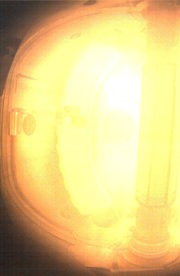
\includegraphics[width=0.13\textwidth]{he-plasama-shape-407.jpg}}
    	%\put(27,39){$\uparrow$}
    	\put(48,60){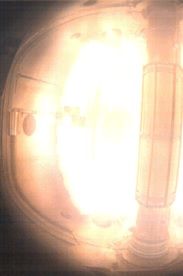
\includegraphics[width=0.13\textwidth]{he-plasama-shape-42.jpg}}
       	%\put(55,52){$\downarrow$}
       	\put(75,60){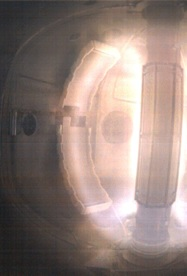
\includegraphics[width=0.13\textwidth]{he-plasama-shape-435.jpg}}
        %\put(80,29){$\downarrow$}
        \put(43,1){\mbox{\colorbox{white}{\hspace{1.5em}时间 ($\rm ms$)}}}
    \end{overpic}
    %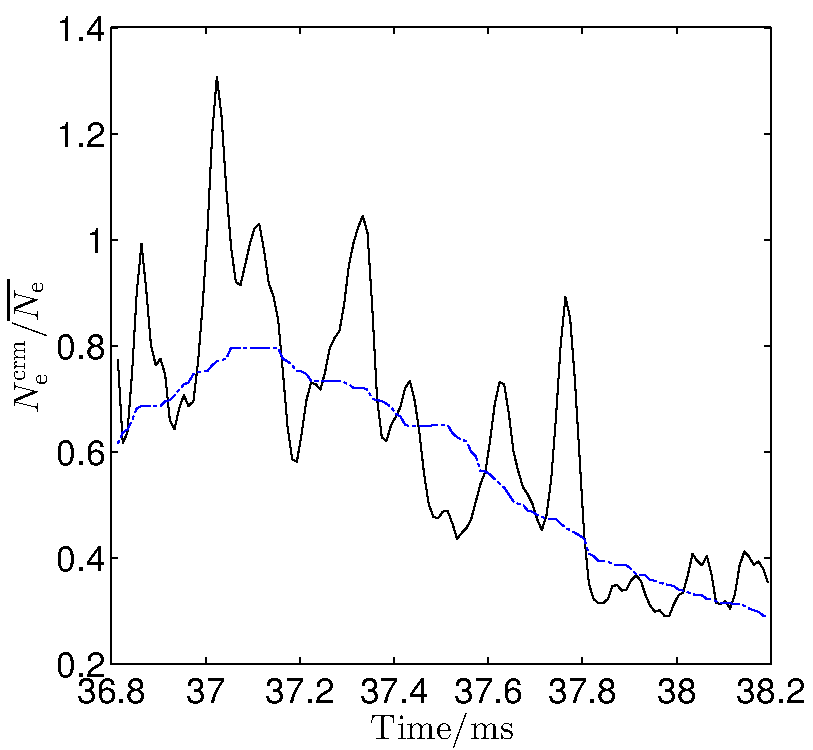
\includegraphics[width=.7\textwidth]{ne-ratio-lineratio-to-mi.pdf}
    \caption{比值 $N_{\rm e}^{\rm crm}/\overline{N_{\rm e}}$ 的实验测量值与高速相机图像。其中点划线为测量值的中值拟合曲线。}%
    \label{fig:chap04:ne-ratio-lineratio-to-mi}
\end{figure}

图 \ref{fig:chap04:ne-te-and-line-intensity-profile}(a) 所示为不同分布参数下,电子密度和电子温度的分布剖面图,分布参数 $\gamma$ 取值越小,电子密度或温度参数的分布越平坦,反之,分布越峰化。图 \ref{fig:chap04:ne-te-and-line-intensity-profile}(b) 所示为当分布参数 $\gamma_{N_{\rm e}}=\gamma_{T_{\rm e}}=1.0$ 时,本文碰撞辐射模型计算的谱线比法用到的三条氦原子谱线的辐射率分布。可见,等离子体中心的谱线辐射率最低,边界辐射率高。这是因为等离子体中心电子温度和密度高,氦原子电离率高,中心的中性粒子总数低;在限制器外,等离子体温度和密度很低,基态原子被激发数量低,辐射率也随之降低。

在特定的等离子体电子密度和温度分布参数下,将等离子体空间谱线辐射率沿测量路径积分,即可对沿路径积分的谱线辐射测量进行模拟计算,进而计算出在不同的分布参数下,谱线比法所得电子密度 $N_{\rm e}^{\rm crm}$ 与弦平均电子密度 $\overline{N_{\rm e}}$ 之间的关系,如图 \ref{fig:chap04:line-int-ratio-params-to-mean-ne} 所示。可见,当 $\gamma_{N_{\rm e}}$ 取值从 $0.5$ 到 $2$ 变化时,谱线比法获得的 $N_{\rm e}^{\rm crm}$ 与弦平均电子密度 $\overline{N_{\rm e}}$ 的比值 $N_{\rm e}^{\rm crm}/\overline{N_{\rm e}}$ 在 $0.8\sim0.3$ 区间变化。$N_{\rm e}^{\rm crm}/\overline{N_{\rm e}}$ 的取值随着电子密度分布参数 $\gamma_{N_{\rm e}}$ 的增加而减小,而 $\gamma_{T_{\rm e}}$ 的取值对 $N_{\rm e}^{\rm crm}/\overline{N_{\rm e}}$ 的变化趋势并无影响,当 $\gamma_{N_{\rm e}}$ 取值大于 $1.5$ 时,此变化关系减弱,甚至消失。

$N_{\rm e}^{\rm crm}/\overline{N_{\rm e}}$ 随 $\gamma_{N_{\rm e}}$ 变化的趋势结合实际测量结果可以对电子密度分布进行定性的诊断。图 \ref{fig:chap04:ne-ratio-lineratio-to-mi} 所示,等离子体放电平顶段实验测量的 $N_{\rm e}^{\rm crm}/\overline{N_{\rm e}}$ 随时间变化曲线以及高速可见光相机拍摄的等离子体图像。可见,在刚进入等离子体平顶段时,随着放电的进行,比值 $N_{\rm e}^{\rm crm}/\overline{N_{\rm e}}$ 自约 $0.8$ 单调下降至约 $0.3$, 结合图 $\ref{fig:chap04:line-int-ratio-params-to-mean-ne}$ 的结果可以得到,在放电平顶段 $\gamma_{N_{\rm e}}$ 自约 $0.5$ 增长至约 $1.5$,电子密度的分布自平坦逐步峰化,这与高速相机图像的测量结果是相符的。而且此测量结果与 SUNIST 的放电经验也是相符的:由于垂直磁场无反馈控制,在放电后期等离子体被急剧压缩\cite{ZengLong2010:Thesis}。

需要注意的是,虽然这种方法只能用来对 $N_{\rm e}$ 分布进行定性的诊断,但可以实现在线的快速实时诊断测量,对于小型托卡马克装置来讲不失为一种低成本快速电子密度分布诊断方法,为今后实现 SUNIST 垂直场的反馈控制提供参考。本方法的局限性在于对等离子体的水平位移无分析诊断能力,如图 $\ref{fig:chap04:ne-ratio-lineratio-to-mi}$ 中所示等离子体放电过程中,等离子体分布峰化的同时向中心柱压缩,要测量此水平位移,则需借助其它诊断手段
\cite{Elahi2011:displacement,Soltwisch1983:plasma-position}。

\subsection{谱线强度涨落的初步研究}
\label{sec:chap04:line-dbp10-fluctuation}

\begin{figure}%[H]
  \centering
  \begin{overpic}[width=0.5\textwidth]{time_frequency_492_vs_dBp10.pdf}
    \put(22.5,1.5){\mbox{\colorbox{white}{\hspace{1.2em}时间}}}
    %\put(0,23){\rotatebox{90}{\mbox{\colorbox{white}{$T_{\rm e}$ ($\rm eV$)\quad}}}}
    %\put(79,17){\rotatebox{90}{\mbox{\colorbox{white}{\color{red}$N_{\rm e}$ $(\times10^{12}\,{\rm cm}^{-3})$\quad}}}}
  \end{overpic}
  %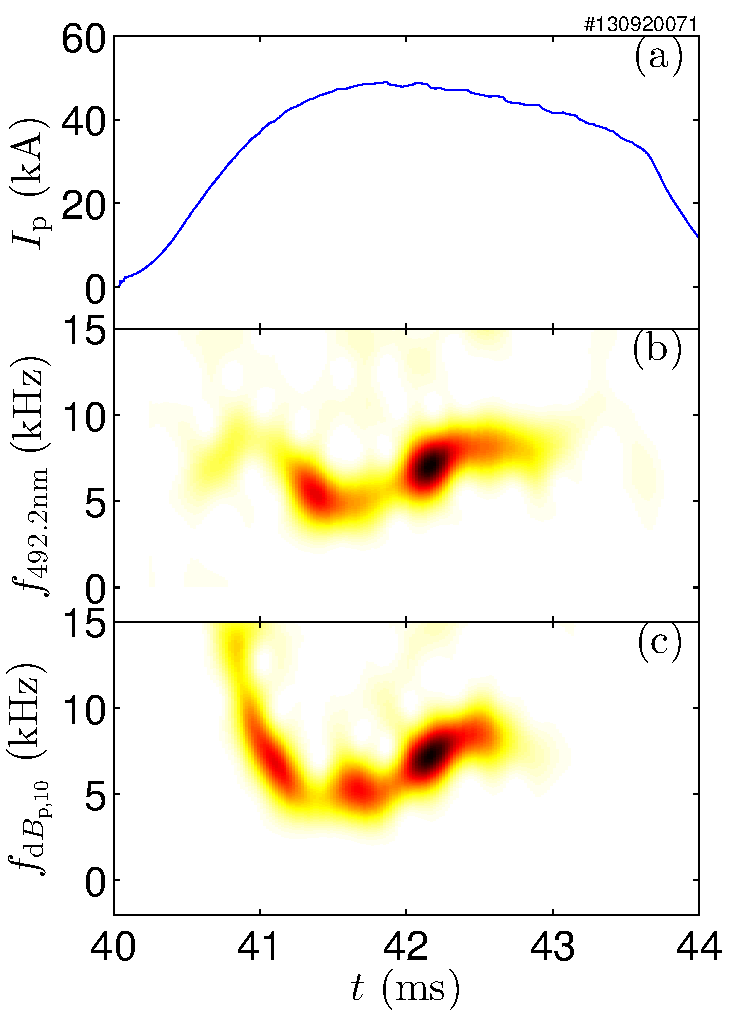
\includegraphics[width=0.6\textwidth]{time_frequency_492_vs_dBp10.pdf}
  \caption{SUNIST 氦等离子体放电 $492.2\,{\rm nm}$ 谱线强度与极向磁探针信号 ${\rm d}B_{{\rm p},10}$ 的扰动的时频分析。(a) 等离子体电流;(b) $492.2\,{\rm nm}$ 谱线强度扰动的功率时频谱图;(c) ${\rm d}B_{{\rm p},10}$ 的扰动的功率时频谱图。(a) 与 (b) 图中分别为各自扰动功率的相对值。}
  \label{fig:chap04:spectromgram-light-dbp10}
\end{figure}

第 \ref{sec:chap04:lineratio-ne-te} 节中我们提到,在测量结果中,谱线强度的涨落造成了谱线比的涨落,从而导致等离子体参数诊断结果的涨落,图 \ref{fig:chap04:spectromgram-light-dbp10} 显示了 SUNIST 氦等离子体放电时 $492.2\,{\rm nm}$ 谱线强度与极向磁探针信号 ${\rm d}B_{{\rm p},10}$ 扰动的时频分析结果。可见,氦原子谱线与极向磁探针信号具有一致的时频功率谱。由此,我们分析光谱强度的涨落可能由以下原因造成:不同的等离子体 $T_{\rm e}$ 和 $N_{\rm e}$ 参数组合对应不同的谱线辐射强度,SUNIST 等离子体的参数具有空间模式结构,等离子体在真空室内旋转,在固定位置测得的谱线强度则呈现周期性涨落。谱线强度的涨落信息体现了等离子体的磁流体力学(MHD)行为,则利用等离子体的光谱信号可以完成其磁流体力学的相关诊断研究工作\cite{MaShuiliang2011:PoP,OES:MHD:1,OES:MHD:2,OES:MHD:3,OES:MHD:4}。对于 SUNIST 等离子体,其内在联系需要更进一步结合电磁诊断信号的研究,由于超出了本文研究范围,这里不再进行深入研究,但此结果为今后丰富光谱诊断工作内容提供了方向和思路。

\section{小结}

基于重复放电测量手段,对 SUNIST 氦等离子体进行了可见光波段氦原子的谱线辐射诊断。本章首先给出了 SUNIST 氦放电等离子体原子发射谱线强度的测量结果,利用谱线比法获得了等离子体的电子温度和密度参数:$T_{\rm e}=90\sim120\,{\rm eV}$,$N_{\rm e}=1.0\sim4.0\times 10^{12}\,{\rm cm}^{-3}$,该诊断结果与微波干涉仪的测量结果相吻合,验证了本文建立的谱线比法的适用性,通过对氦原子激发态数密度的研究对碰撞辐射模型进行了再次核验。

由于光谱诊断测量具有弦积分特性,而光谱辐射与电子温度和密度是非线性关系,导致谱线比和微波干涉仪对电子密度诊断之间特定的比值关系。通过对电子分布参数进行抛物线分布的假设计算,获得了两诊断方法结果的比值关系,利用此比值关系给出了一种可以用于定性诊断等离子体电子密度空间分布的诊断手段。同时,研究还观察到氦原子的谱线辐射强度涨落与磁探针信号具有一致的时频行为特性,由此我们推测氦原子的谱线辐射也携带了大量的等离子体磁流体力学行为信息。这些都为今后进一步丰富和深入 SUNIST 的光谱诊断研究工作提供了参考。
